\chapter{CUORE}

CUORE (Cryogenic Underground Observatory for Rare Events) is located in Gran Sasso, Italy, and utilizes a bolometric method to search for \zeronubb. The experiment will run with 988 crystals of TeO$_2$ held at roughly 10 mK. The source of \zeronubb~are the $^{130}$Te nuclei inside of the crystals ($34.2\%$ natural abundance \cite{Fehr200483}). Thus, in this setup, the crystals act as both sources and detectors of \zeronubb. When energy is deposited in the crystals, such as from the electrons emitted during \zeronubb, the temperature of the crystals rises. The Q-value of the decay of interest, viz. $^{130}\textrm{Te} \rightarrow ^{130}\textrm{Xe} + e + e$, is $2527.518\pm 0.013$ keV \cite{Redshaw:2009cf}\cite{Scielzo:2009nh}\cite{Rahaman:2011zz}. This high Q-value is well-separated from other naturally occurring environmental $\gamma$'s except for $^{60}$Co at 2506 keV and $^{208}$Tl at 2615 keV. However, the resolution of the CUORE crystals is $7.7\pm0.5$ keV, which means that these peaks do not significantly worsen the background in the region of interest at the Q-value. In addition, this resolution aids in understanding background sources that deposit energy the detector as each \gamma~line can be observed above the Compton background, which aids in identifying particular background sources.

\section{CUORE Detectors}

\subsection{Particle Detection with Bolometers}
As noted in \autoref{sec:State of Neutrinoless Double Beta Decay Experiments}, current experiments in the field of \zeronubb~use a wide array of technologies to identify \zeronubb~events. However, CUORE utilizes a different method of calorimetry than its counterparts in that it uses what is known as the bolometric method. As particles pass through matter, the energy they deposit is eventually carried into the surrounding material as heat. This method requires a mass that acts as a thermal capacitor, a weak thermal connection to a heat bath, and a thermometer (generally a thermistor) and CUORE's setup is sketched in \autoref{fig:thermal_crystal_cartoon} and a sample pulse is shown in \autoref{fig:Sample_pulse}. The detectors in CUORE, $\textrm{TeO}_2$~crystals, respond to energy deposition by a temperature rise according to
\begin{equation}
\delta T = \delta E/C(T).
\end{equation}
At low C, $\delta T$ is maximized; therefore, the crystals are operated at low temperatures where C(T) is given by the Debye Model:
\begin{equation}
C(T)\sim T^3.
\end{equation} 
This temperature dependence on the heat capacity is what drives the need for low temperatures the CUORE detectors all the way down to $\sim10$ mK. The custom cryostat used to do this is described later on in \autoref{sec:CUORE Cryostat}. At these temperatures, the heat capacity of the crystals in CUORE is $2\times 10^{-9} \textrm{J/K}$

\begin{figure}[htbp]
\centering
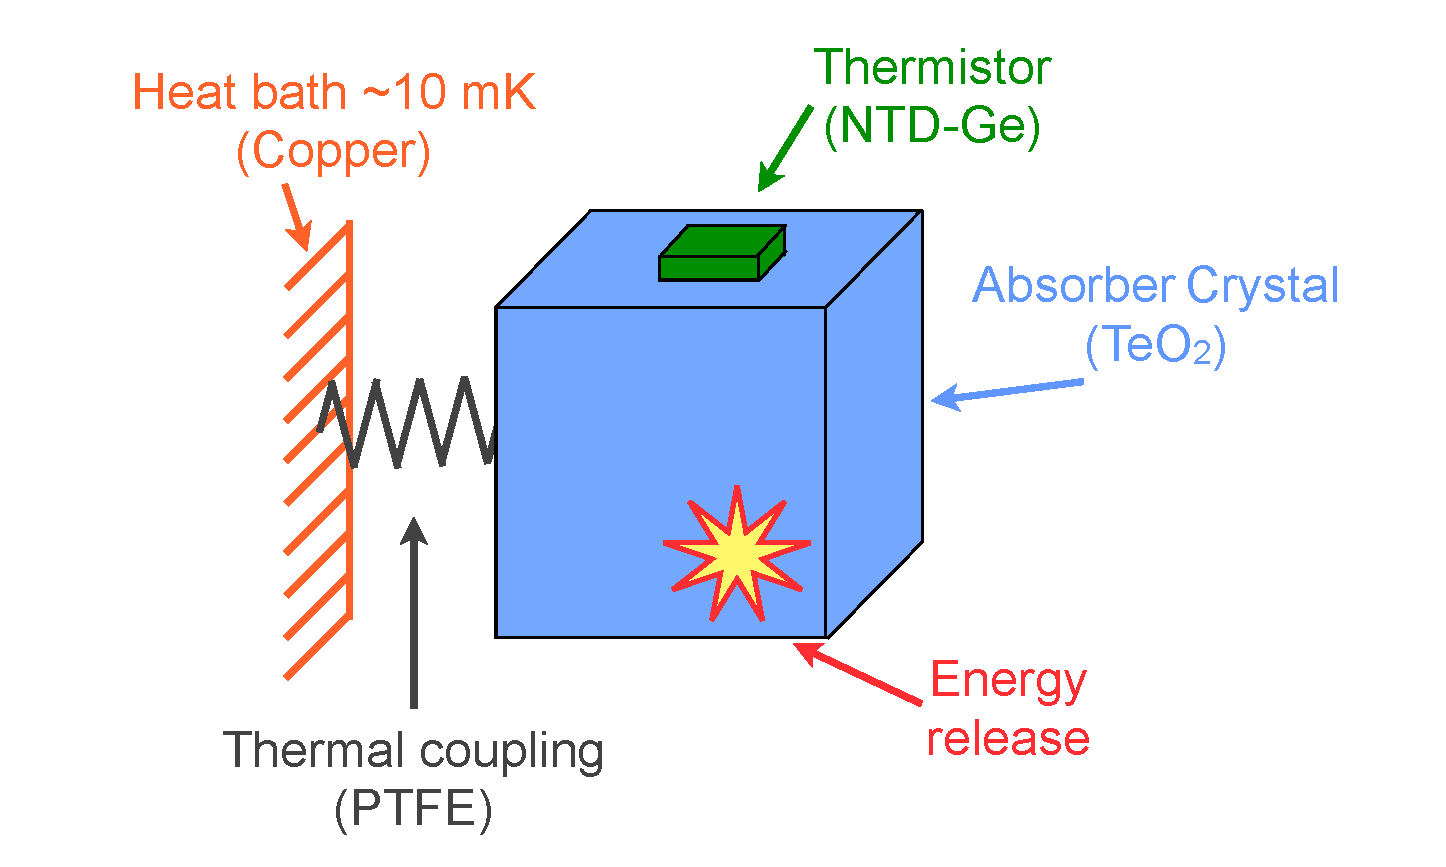
\includegraphics[width=0.7\linewidth]{Figures/bolosketch-color.pdf}
\caption[A diagram of the thermal connection of the TeO$_2$ crystals to the thermal bath provided by the copper frames.]{A diagram of the thermal connection of the TeO$_2$ crystals to the thermal bath provided by the copper frames. The weak thermal coupling is provided by the PTFE.}
\label{fig:thermal_crystal_cartoon}
\end{figure}

\begin{figure}[htbp]
\centering
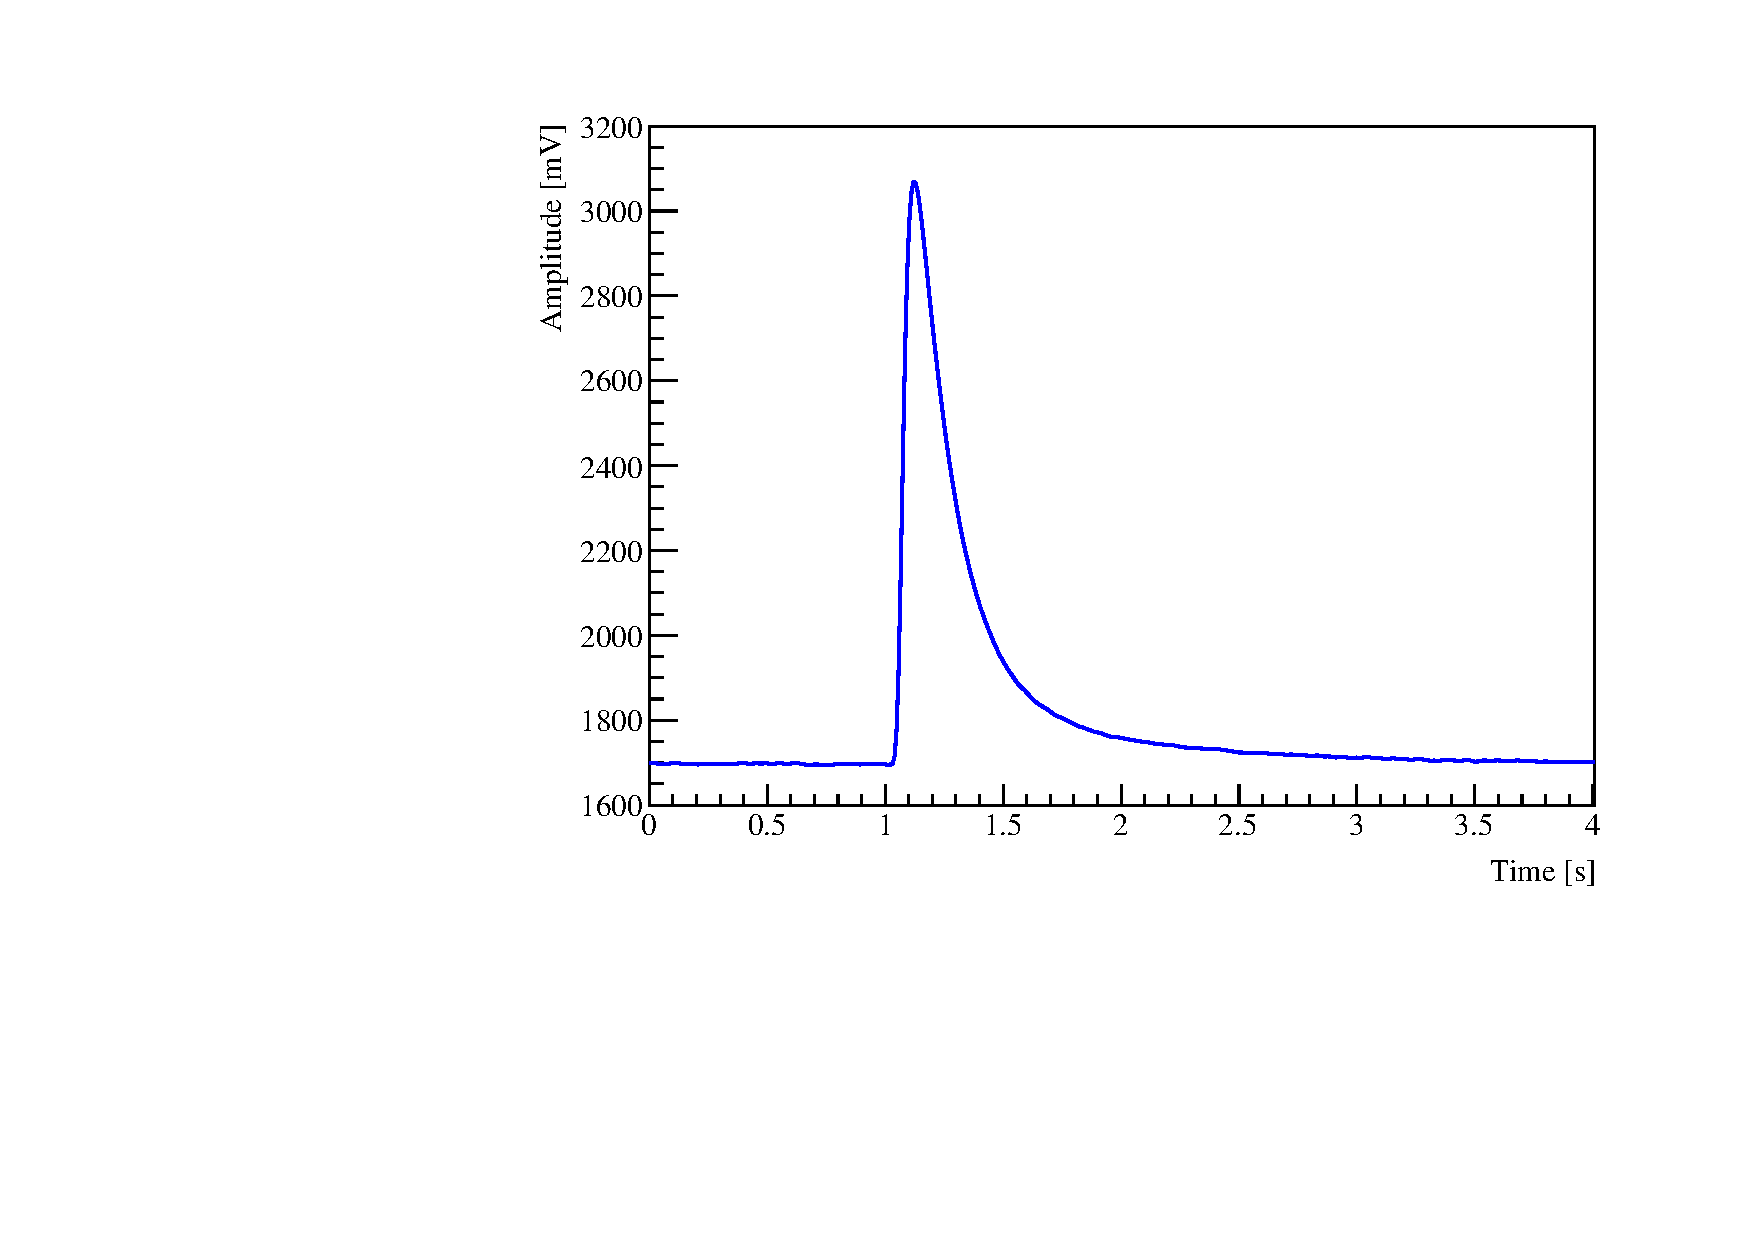
\includegraphics[width=0.7\linewidth]{Figures/pulse-conference.pdf}
\caption[An example pulse from a single CUORE detector.]{An example pulse from a single CUORE detector. After an event at 1 s where energy is deposited in the crystal, a fast temperature rise is observed along with a slow cooling through the weak thermal coupling.}
\label{fig:Sample_pulse}
\end{figure}

\subsection{CUORE Detector Array}

\section{Predecessor Experiments}

\subsection{Cuoricino}

\subsection{CUORE-0}

\section{CUORE Cryostat}
\label{sec:CUORE Cryostat}

Since the heat capacity of the CUORE crystals is so strongly dependent on temperature, it is important to have a system that can cool down the crystals to low temperatures and keep them running in stable conditions over long periods. To this end, we constructed a custom cryostat to house the crystals. The cooling components of the cryostat are pulse tubes that cools the cryostat stages held 4 K and a dilution refrigerator that is responsible for maintaining the coldest regions of the cryostat, including the crystals at 10 mK. In addition to cooling the crystals, the cryostat also houses the shielding for the crystals and, since this is a low-background experiment, needs to be made of radiopure materials, especially near the detectors themselves.

\begin{figure}[htbp]
\centering
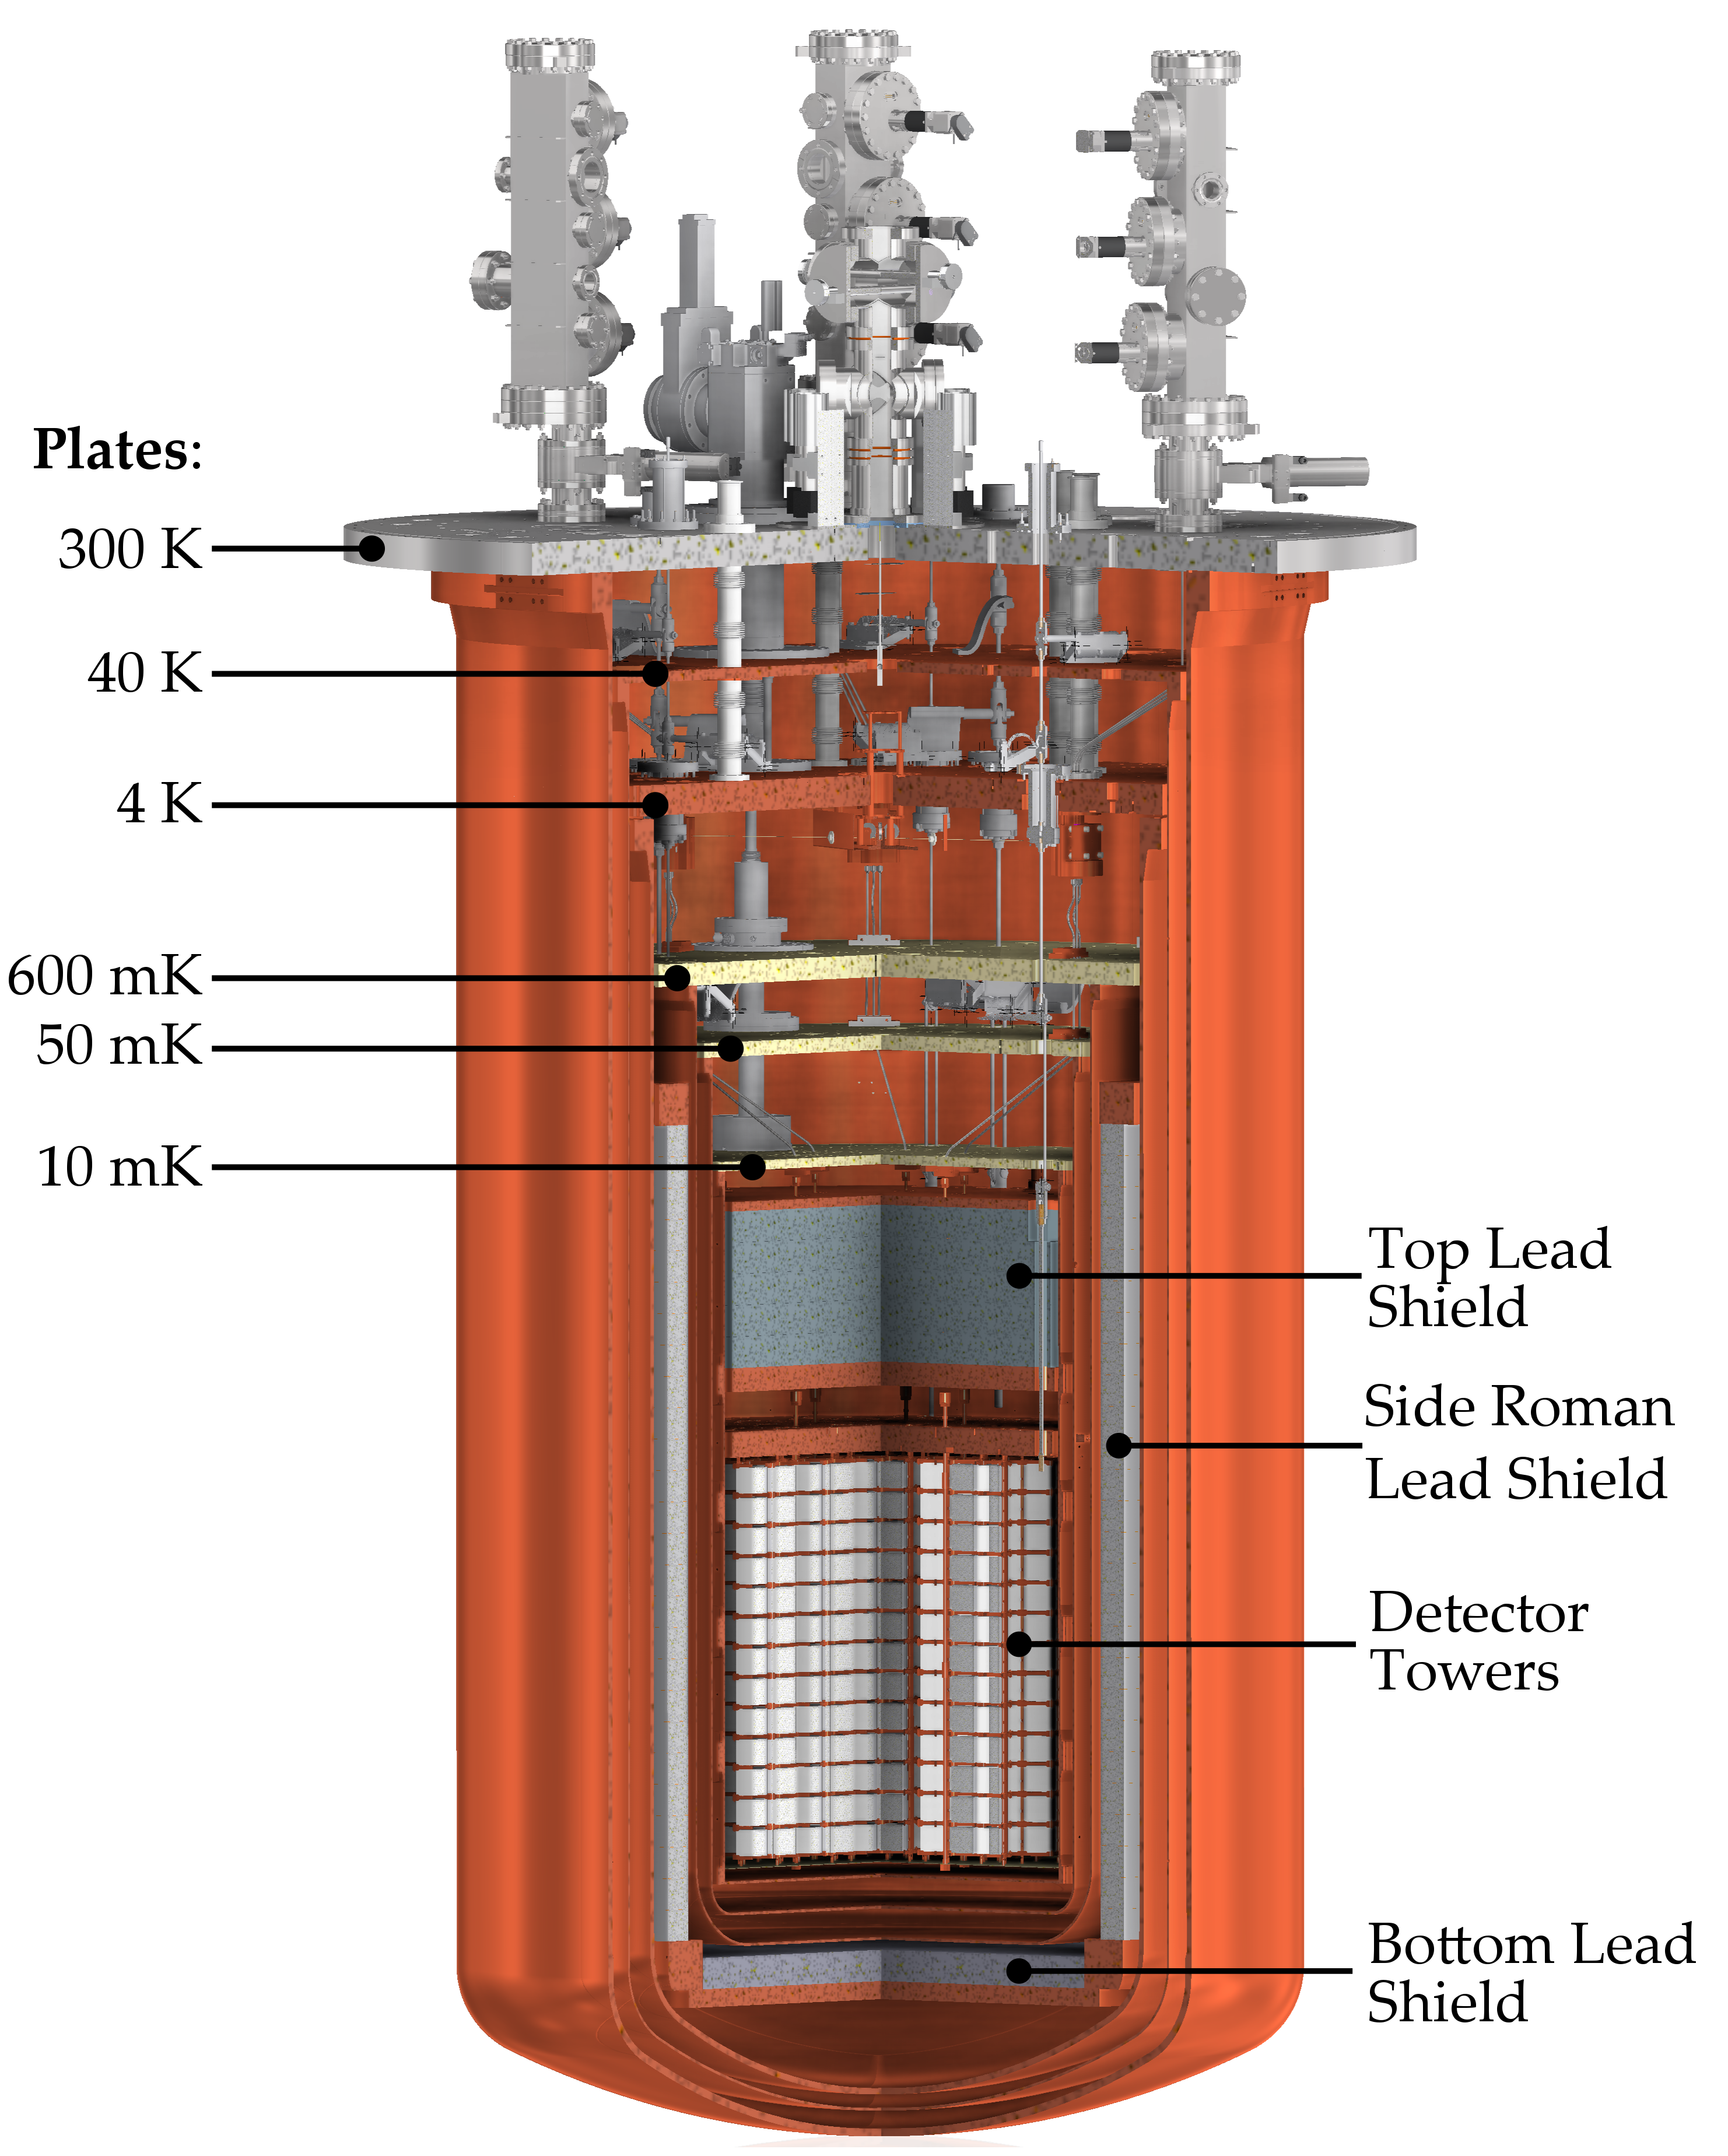
\includegraphics[width=\linewidth]{Figures/cryostat_Adjusted.png}
\caption{A CAD drawing of a cutaway the CUORE cryostat showing the internal shielding of the cryostat. The temperature stages of the cryostat are also shown. Not included are the external shields which extend around the sides of the cryostat}
\label{fig:cryostat_cad_cutout}
\end{figure}

\subsubsection*{Cooling Systems}

Since the cyrostat needs to reach temperatures of 10 mK, a dilution refrigerator is used as the main cooling mechanism in the coldest stages of the cryostat. A dilution refrigerator works by diluting a He-3 solution \color{red}Add more here!\color{black}.

\subsubsection*{Radiopurity}

\begin{figure}[htbp]
\centering
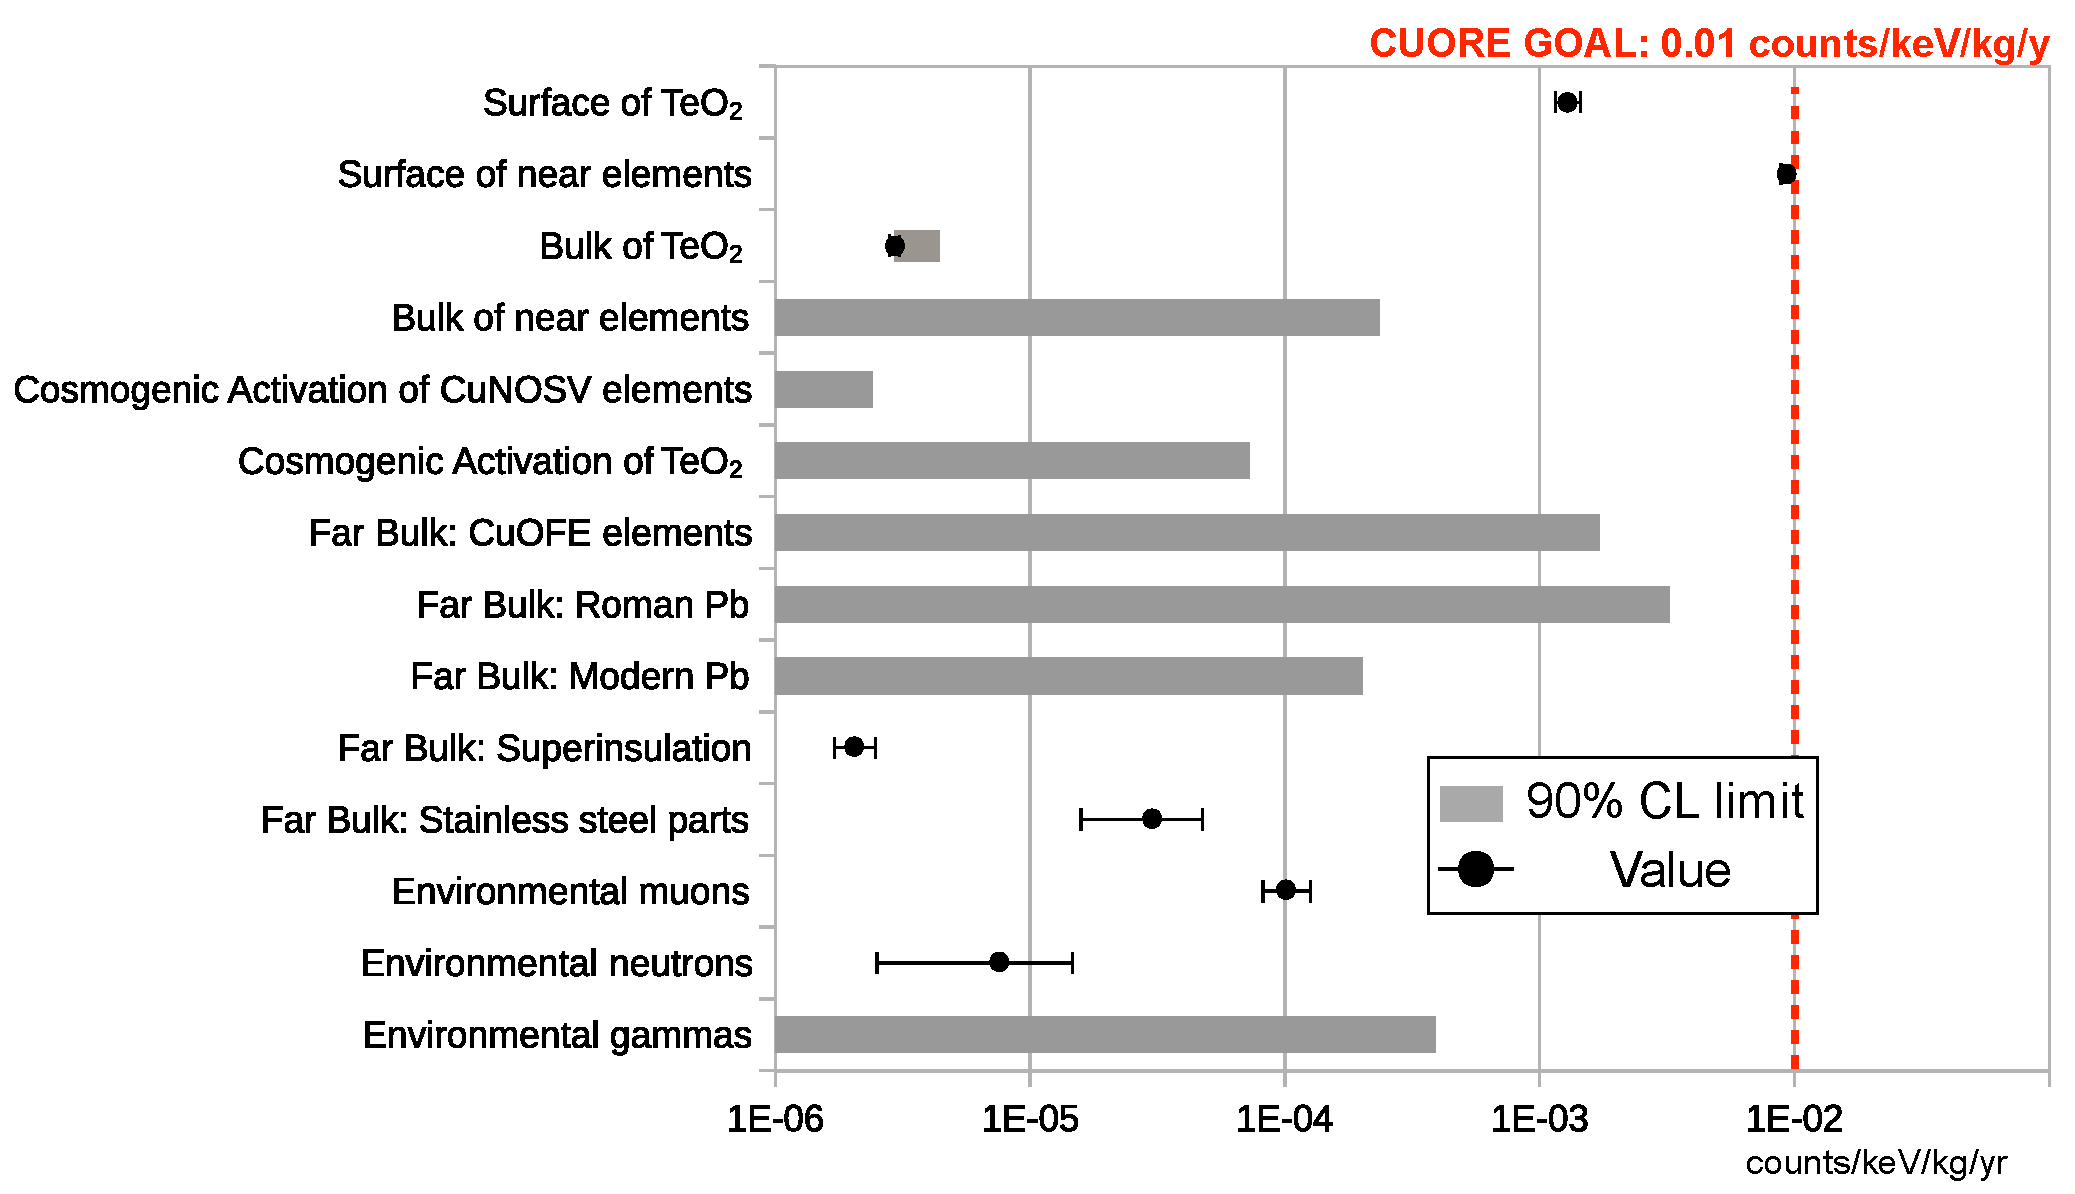
\includegraphics[width=0.7\linewidth]{Figures/CUORE_background_budget}
\caption{CUORE background budget. The CUORE goal is 0.01 counts/keV/kg/y with most of the background due to the surfaces of cryostat elements nearest to the crystal and the bulk of the Roman lead.}
\label{fig:istogramma}
\end{figure}

The background goal of CUORE is to have no greater than 0.01 counts/keV/kg/yr in the region of interest, defined to be a 100 keV interval from 2470 keV to 2570 keV. In order to achieve this low background, the parts nearest to the detectors undergo intensive cleaning. The contamination of these surfaces is given in \autoref*{tab:NearDetectorSources}.

\begin{table}[htbp]
\centering
\caption[90\% upper limits of $^{232}$Th and $^{238}$U bulk contamination of sources near the detector.]{90\% upper limits of $^{232}$Th and $^{238}$U bulk contamination of sources near the detector. Table from \cite{Alduino:2016vjd}}
\label{tab:NearDetectorSources}
\begin{tabular}{|c|c|c|}
\hline 
 Component & $^{232}$Th [g/g] & $^{238}$ U [g/g] \\ 
\hline 
TeO$_2$ crystals & $< 2.1\times 10^{-13}$ & $<5.3\times 10^{-14}$ \\ 
\hline 
NOSV copper & $<5.0 \times 10^{-13}$ & $<5.3 \times 10^{-12}$ \\ 
\hline 
NTD sensors & $< 1.0 \times 10^{-9}$ & $<1.0 \times 10^{-9}$ \\ 
\hline 
Bonding gold wires & $< 1.0 \times 10^{-8}$ & $<1.0 \times 10^{-9}$ \\ 
\hline 
Si heaters &   $<8\times 10^{-11}$ & $<1.7 \times 10^{-10}$ \\ 
\hline 
PTFE holders & $<1.5\times 10^{-12}$ & $<1.8 \times 10^{-12}$ \\ 
\hline 
Cu-PEN cables & $<4.4\times 10^{-10}$ & $<1.1 \times 10^{-10}$ \\ 
\hline
Glue & $<2.2\times 10^{-10}$ & $<8.2\times10^{-10}$ \\
\hline 
\end{tabular} 
\end{table}



\begin{comment}

\subsection{CUORE Detectors}

The CUORE detectors are 988 $ 5\times 5 \times 5~ \textrm{cm}^3$ crystals arranged into 19 towers with 13 floors containing 4 crystals each as shown in \hyperref[fig:cuore-detector-array0]{Fig. \ref*{fig:cuore-detector-array0}}. The total detector mass is 742 kg with 206 kg of $^{130}$Te. 

\begin{figure}[htbp]
\centering
\includegraphics[width=0.7\linewidth]{"Figures/CUORE detector array_0"}
\caption{A rendering of the CUORE towers. The 19 towers are arranged into rows of 3, 4, 5, 4, and 3 towers.}
\label{fig:cuore-detector-array0}
\end{figure}


The crystals in each tower are held by copper frames, with polytetrafluoroethylene (PTFE) in between the copper and the crystals. The crystals respond to energy deposition by a small temperature rise according to
\begin{equation}
\delta T = E/C(T).
\end{equation}
At low C, $\delta T$ is maximized; therefore, the crystals are operated at low temperatures where C(T) is given by the Debye Model:
\begin{equation}
C(T)\sim T^3.
\end{equation}
At 10 mK, the operating temperature of CUORE, the heat capacity is $\sim2$ nJ/K, which causes a 1 MeV energy deposit to have a $\delta T$ of $\sim0.1$ mK.

This temperature rise is measured by a neutron-transmutation-doped (NTD) germanium thermistors which are glued onto each crystal. These thermistors allow the temperature change of the crystals to be read out by electronics as a change in applied voltage. Also glued on the crystals are silicon resistors which are used as a Joule heater. Bonded to the thermistors and the heaters are gold wires which are bonded to copper tape with a polyethylene naphthalate (PEN) substrate (collectively called Cu-PEN) on wire trays along the sides of the towers, shown in \hyperref[fig:bondedchips]{Fig. \ref*{fig:bondedchips}}.
\begin{figure}[htbp]
\centering
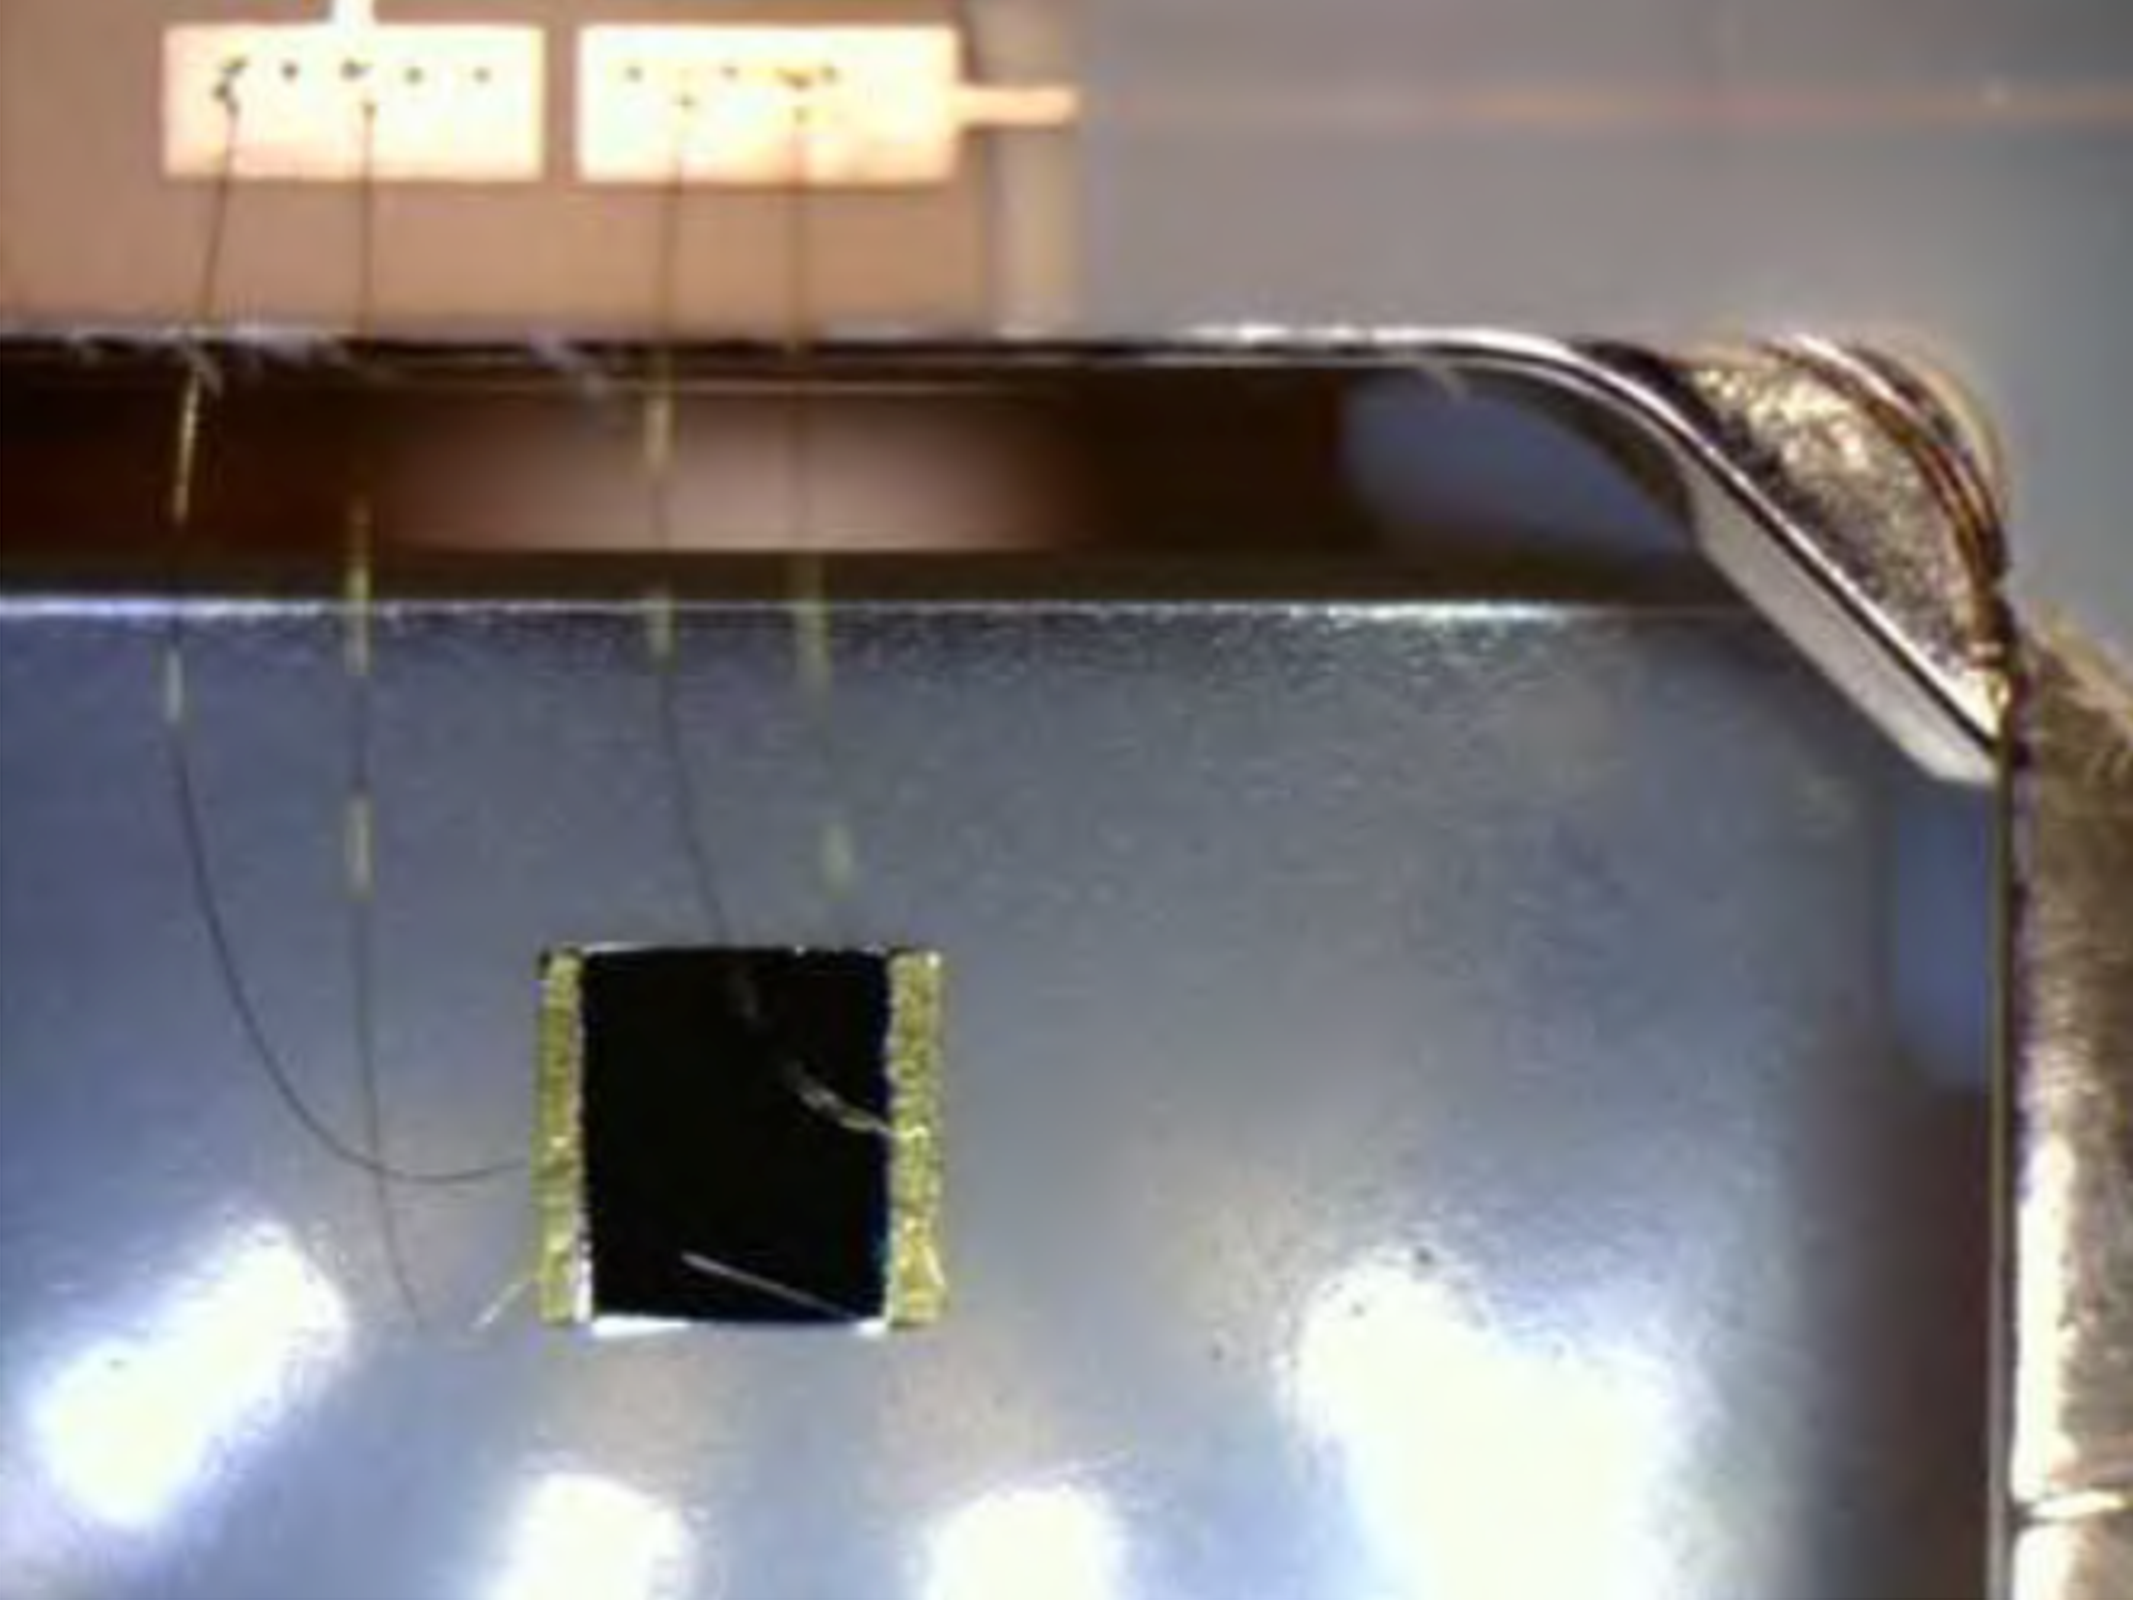
\includegraphics[width=0.7\linewidth]{Figures/BondedChips}
\caption{A germanium NTD on the crystal with four gold wires that have been bonded to both the NTD and to copper pads on the Cu-PEN tape.}
\label{fig:bondedchips}
\end{figure}
These signals are then read out by room-temperature electronics on top of the cryostat. A rendering of a full tower with the copper frames, wire trays, PTFE, and crystals can be seen at \hyperref[fig:SingleTowerWithZoom]{Fig. \ref*{fig:SingleTowerWithZoom}}

\begin{figure}[htbp]
\centering
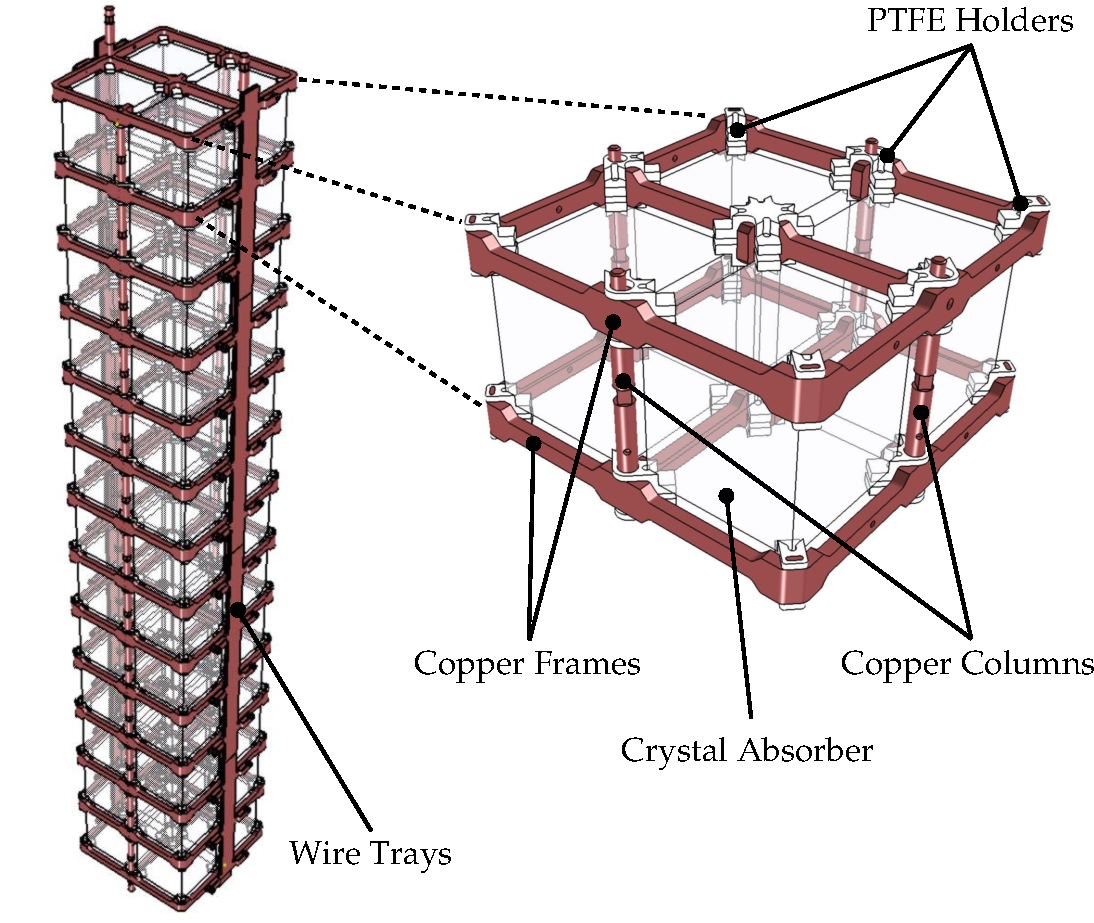
\includegraphics[width=0.7\linewidth]{Figures/C0TowerZoom.pdf}
\caption[A rendering of a single tower in the CUORE detector assembly with a cutout for a single floor. Adjacent floors share the same frames.]{A rendering of a single tower in the CUORE detector assembly with a cutout for a single floor. Adjacent floors share the same frames. Diagram from \cite{Alduino:2016vjd}}
\label{fig:SingleTowerWithZoom}
\end{figure}

After an energy deposition causes the temperature of the crystal to rise, the crystal returns slowly back to the baseline temperature due to the weak thermal connection between the crystals and the copper frames which are held at 10 mK. A diagram of the thermal connection is shown in \hyperref[fig:thermal_crystal_cartoon]{Fig. \ref*{fig:thermal_crystal_cartoon}}. The rise and fall times of the signal are around 0.05 seconds and 0.2 seconds, respectively, for a 2615 keV signal.

\begin{figure}[htbp]
\centering
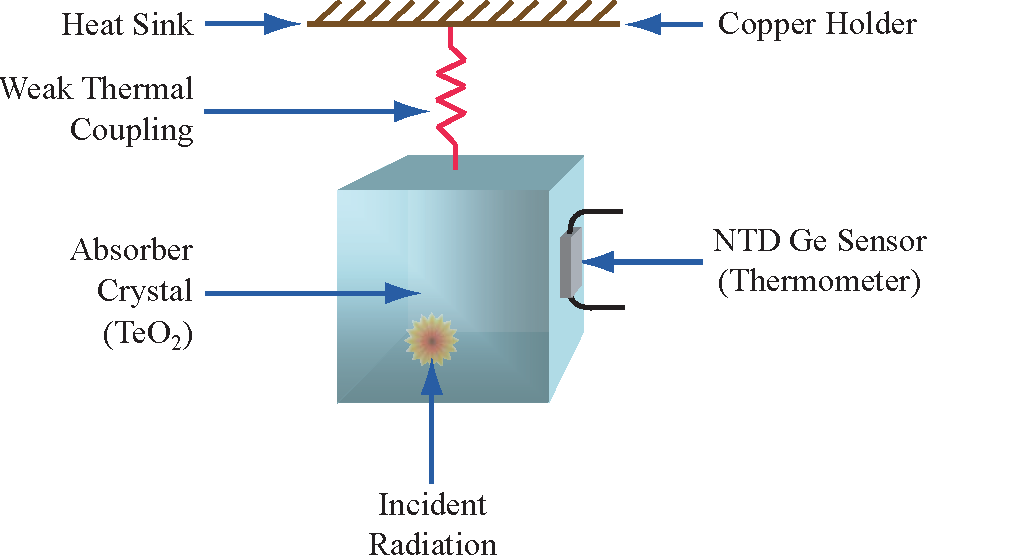
\includegraphics[width=0.7\linewidth]{Figures/BolDetector_Cartoon.pdf}
\caption[A diagram of the thermal connection of the TeO$_2$ crystals to the thermal bath provided by the copper frames. The weak thermal coupling is provided by the PTFE and the gold wires for the NTD and the heater. The thermistor is not shown to scale.]{A diagram of the thermal connection of the TeO$_2$ crystals to the thermal bath provided by the copper frames. The weak thermal coupling is provided by the PTFE and the gold wires for the NTD and the heater. The thermistor is not shown to scale. Diagram from \cite{Alduino:2016vjd}}
\label{fig:thermal_crystal_cartoon}
\end{figure}



\subsection{CUORE Cryostat}

Since the heat capacity of the CUORE crystals is so strongly dependent on temperature, it is important to have a system that can cool down the crystals to low temperatures and keep them running in stable conditions over long periods. To this end, we constructed a custom cryostat to house the crystals. The cooling components of the cryostat are pulse tubes that cools the cryostat stages held 4 K, and a dilution refrigerator that is responsible for maintaining the coldest regions of the cryostat, including the crystals at 10 mK. In addition to cooling the crystals, the cryostat also houses the shielding for the crystals and needs to be made of radiopure materials, especially near the detectors themselves.

\begin{figure}[htbp]
\centering
\includegraphics[width=\linewidth]{Figures/Cryostat_Adjusted.png}
\caption{A CAD drawing of a cutaway the CUORE cryostat showing the internal shielding of the cryostat. The temperature stages of the cryostat are also shown. Not included are the external shields which extend around the sides of the cryostat}
\label{fig:cryostat_cad_cutout}
\end{figure}

\subsubsection*{Cooling Systems}

Since the cyrostat needs to reach temperatures of 10 mK, a dilution refrigerator is used as the main cooling mechanism in the coldest stages of the cryostat. A dilution refrigerator works by diluting a He-3 solution
%The CUORE cryostat 

\subsubsection*{Radiopurity}

\begin{figure}[htbp]
\centering
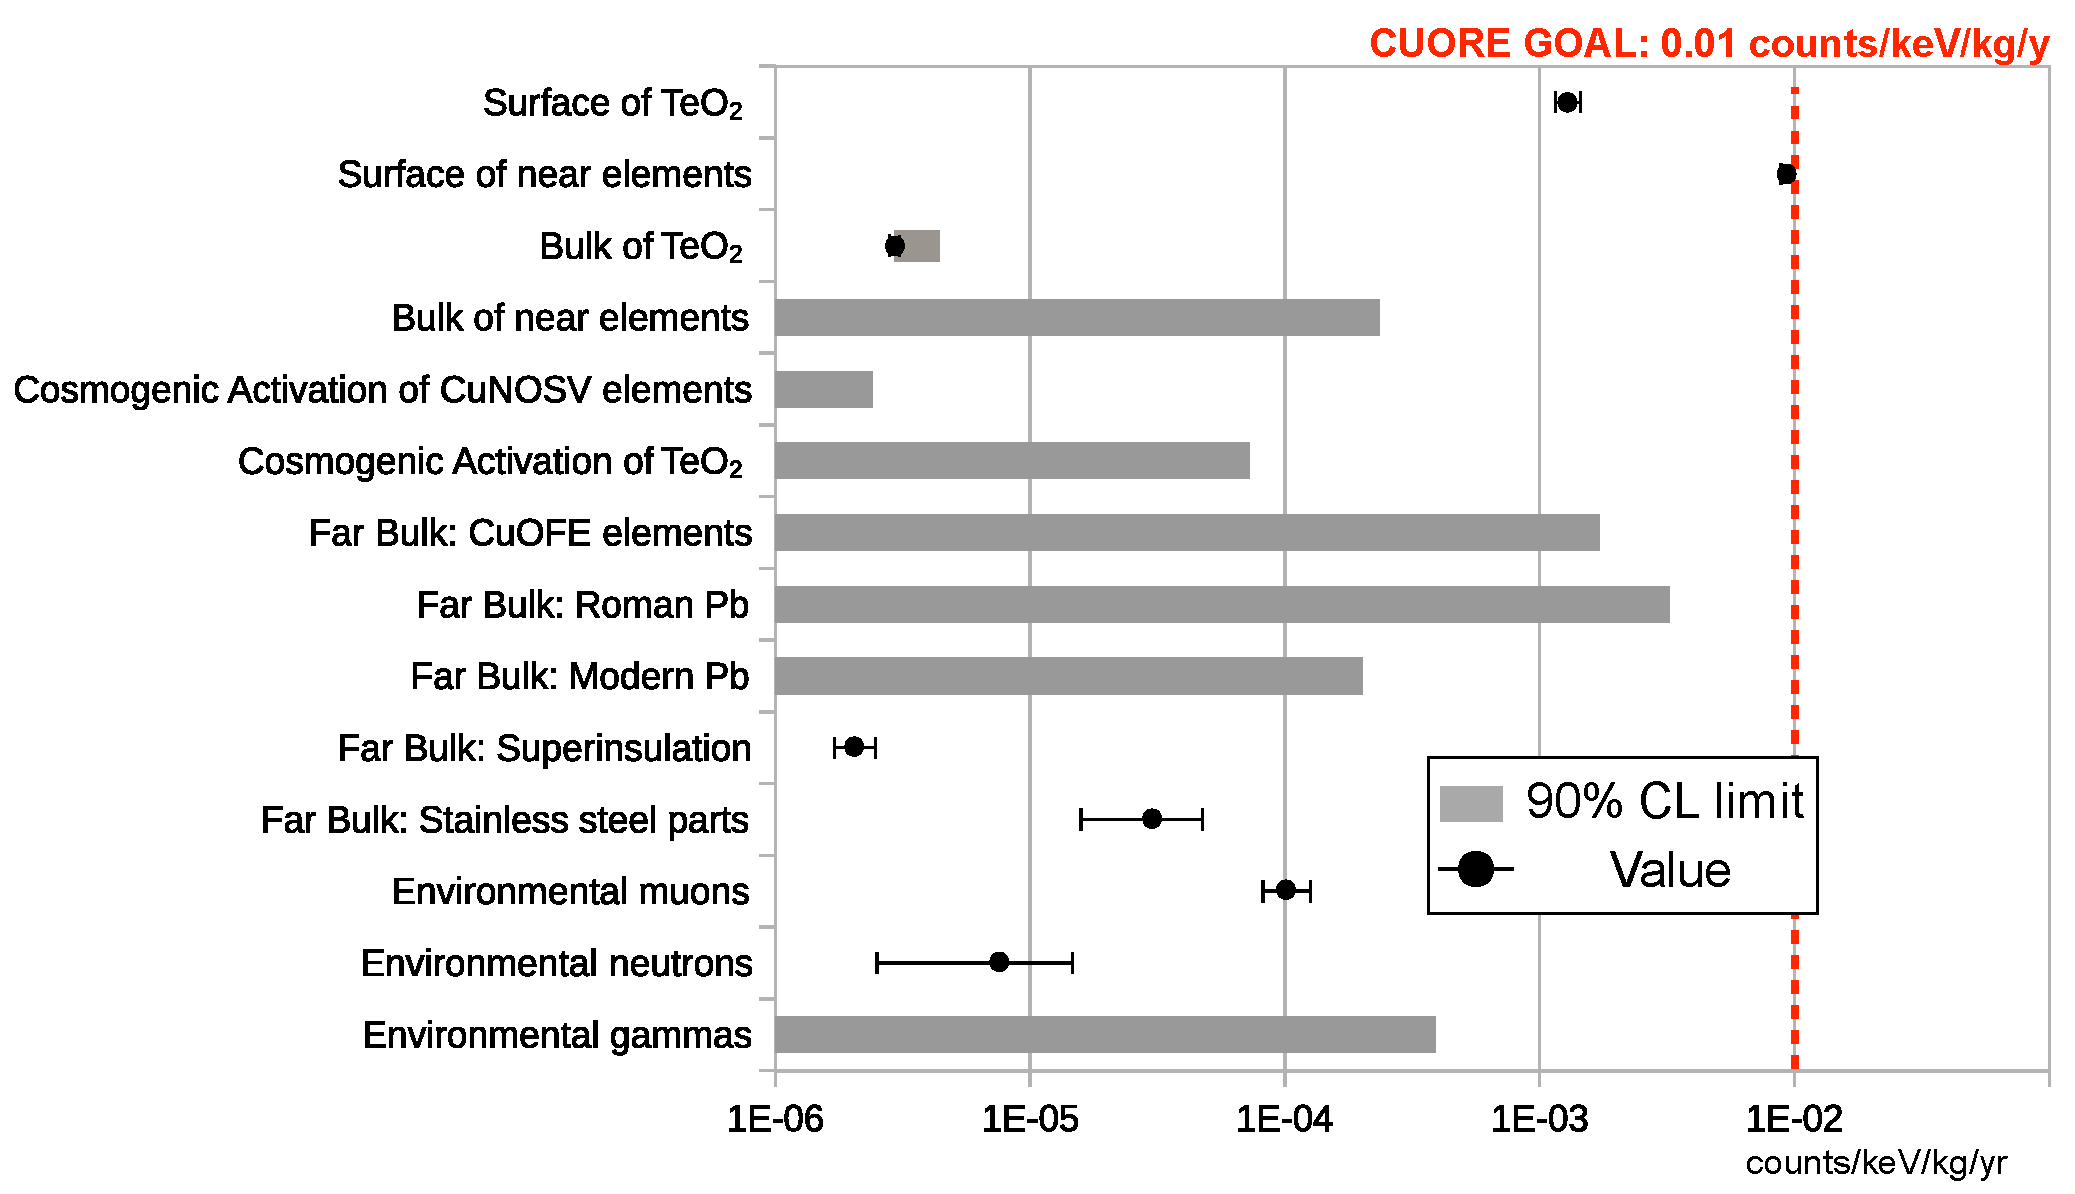
\includegraphics[width=0.7\linewidth]{Figures/CUORE_background_budget}
\caption{CUORE background budget. The CUORE goal is 0.01 counts/keV/kg/y with most of the background due to the surfaces of cryostat elements nearest to the crystal and the bulk of the Roman lead.}
\label{fig:istogramma}
\end{figure}

The background goal of CUORE is to have no greater than 0.01 counts/keV/kg/yr in the region of interest, defined to be a 100 keV interval from 2470 keV to 2570 keV. In order to achieve this low background, the parts nearest to the detectors undergo intensive cleaning. The contamination of these surfaces is given in \hyperref[tab:NearDetectorSources]{Table \ref*{tab:NearDetectorSources}}.

\begin{table}[htbp]
\centering
\caption[90\% upper limits of $^{232}$Th and $^{238}$U bulk contamination of sources near the detector.]{90\% upper limits of $^{232}$Th and $^{238}$U bulk contamination of sources near the detector. Table from \cite{Alduino:2016vjd}}
\label{tab:NearDetectorSources}
\begin{tabular}{|c|c|c|}
\hline 
 Component & $^{232}$Th [g/g] & $^{238}$ U [g/g] \\ 
\hline 
TeO$_2$ crystals & $< 2.1\times 10^{-13}$ & $<5.3\times 10^{-14}$ \\ 
\hline 
NOSV copper & $<5.0 \times 10^{-13}$ & $<5.3 \times 10^{-12}$ \\ 
\hline 
NTD sensors & $< 1.0 \times 10^{-9}$ & $<1.0 \times 10^{-9}$ \\ 
\hline 
Bonding gold wires & $< 1.0 \times 10^{-8}$ & $<1.0 \times 10^{-9}$ \\ 
\hline 
Si heaters &   $<8\times 10^{-11}$ & $<1.7 \times 10^{-10}$ \\ 
\hline 
PTFE holders & $<1.5\times 10^{-12}$ & $<1.8 \times 10^{-12}$ \\ 
\hline 
Cu-PEN cables & $<4.4\times 10^{-10}$ & $<1.1 \times 10^{-10}$ \\ 
\hline
Glue & $<2.2\times 10^{-10}$ & $<8.2\times10^{-10}$ \\
\hline 
\end{tabular} 
\end{table}


\end{comment}